\documentclass[conference]{IEEEtran}

\usepackage{afterpage}
\usepackage{cite}
\usepackage{graphicx}
\usepackage{url}
\usepackage{amsmath,amssymb,amsfonts}
\usepackage[latin1]{inputenc}
\usepackage[T1]{fontenc}

\ifCLASSINFOpdf
  % \usepackage[pdftex]{graphicx}
  % declare the path(s) where your graphic files are
  % \graphicspath{{../pdf/}{../jpeg/}}
  % and their extensions so you won't have to specify these with
  % every instance of \includegraphics
  % \DeclareGraphicsExtensions{.pdf,.jpeg,.png}
\else
  % or other class option (dvipsone, dvipdf, if not using dvips). graphicx
  % will default to the driver specified in the system graphics.cfg if no
  % driver is specified.
  % \usepackage[dvips]{graphicx}
  % declare the path(s) where your graphic files are
  % \graphicspath{{../eps/}}
  % and their extensions so you won't have to specify these with
  % every instance of \includegraphics
  % \DeclareGraphicsExtensions{.eps}
\fi

\newcommand{\etp}{\textsc{Elus Transport Protocol}}
\newcommand{\ETP}{\textsc{Etp}}
\newcommand{\proxy}{\textsc{Proxy}}
\newcommand{\agent}{\textsc{Agent}}
\newcommand{\adapter}{\textsc{Adapter}}
\newcommand{\scenario}{\textsc{Scenario}}
\newcommand{\handle}{\textsc{Handle}}
\newcommand{\stub}{\textsc{Stub}}
\newcommand{\msg}{\textsc{Message}}
\newcommand{\ELUS}{\textsc{Elus}}
\newcommand{\elus}{\textsc{Epos Live Update System}}
\newcommand{\epos}{\textsc{Embedded Parallel Operating System}}
\newcommand{\EPOS}{\textsc{Epos}}

\usepackage{listings}
\lstset{keywordstyle=\bfseries, flexiblecolumns=true}
\lstloadlanguages{[ANSI]C++,HTML}
\lstdefinestyle{prg} {basicstyle=\footnotesize, lineskip=-0.2ex, showspaces=false,breaklines=true,showstringspaces=false,numbers=left,numbersep=-5pt,frame=single,stepnumber=1}

\newcommand{\prg}[3][tbp]{
  \begin{figure}[#1]
      \lstinputlisting[language=C++,style=prg]{fig/#2.cc}
    \caption{#3\label{prg:#2}}
  \end{figure}
}

\newcommand{\fig}[4][tb]{
  \begin{figure}[#1] {\centering{\includegraphics[#4]{fig/#2}}\par}
    \caption{#3\label{fig:#2}}
  \end{figure}
}

\newcommand{\figspan}[4][tb]{
  \begin{figure*}[#1] {\centering{\includegraphics[#4]{fig/#2}}\par}
    \caption{#3\label{fig:#2}}
  \end{figure*}
}

\newcommand{\tab}[3][th]{
  \begin{table}[#1]
    {\centering\small\textsf{\input{fig/#2.tab}}\par}
    \caption{#3\label{tab:#2}}
  \end{table}
}


% correct bad hyphenation here
\hyphenation{op-tical net-works semi-conduc-tor}

\sloppy

\begin{document}
%
% paper title
% can use linebreaks \\ within to get better formatting as desired
\title{ELUS: a Dynamic Software Reconfiguration Infrastructure for Embedded Systems}


% author names and affiliations
% use a multiple column layout for up to three different
% affiliations
\author{\IEEEauthorblockN{Giovani Gracioli and Ant�nio Augusto Fr�hlich}
\IEEEauthorblockN{Laboratory for Software and Hardware Integration (LISHA)\\
Federal University of Santa Catarina (UFSC)\\
P.O.Box 476, 88040900 -- Florian\'opolis -- Brazil\\
\{giovani,guto\}@lisha.ufsc.br}
}

% make the title area
\maketitle

\begin{abstract}

Dynamic software reconfiguration is the process of updating the system software during its execution. A dynamic software reconfiguration mechanism for an embedded system must be simple, transparent to applications, and use the minimum amount of resources (e.g. memory, processing) possible, since it shares resources with the target embedded system. We present \elus{} (\ELUS{}), an operating system infrastructure for resource-constrained embedded systems. Through the use of sophisticated C++ static metaprogramming techniques, unlike the previous software reconfiguration infrastructures, \ELUS{} provides a low-overhead, simple,
configurable, and fully transparent software reconfiguration mechanism. Our experimental evaluation shows that the \ELUS{} memory consumption, overhead, and reconfiguration time present better performance when compared to related work.

\end{abstract}

% For peer review papers, you can put extra information on the cover
% page as needed:
% \ifCLASSOPTIONpeerreview
% \begin{center} \bfseries EDICS Category: 3-BBND \end{center}
% \fi
%
% For peerreview papers, this IEEEtran command inserts a page break and
% creates the second title. It will be ignored for other modes.
%\IEEEpeerreviewmaketitle


\section{Introduction}

Dynamic software reconfiguration is a desirable feature present in the majority of current systems, from conventional environment computing (e.g. personal computers) to embedded systems. This characteristic allows the system software to be replaced at execution time, in order to correct bugs, add and/or remove features, and adapt the system to varying execution environments.

Wireless Sensor Networks, for example, can comprise a large number of small sensors scattered throughout a
given environment, with few kilobytes of memory and low processing power~\cite{asada98wireless}. Very often, collecting such sensors for in-lab reprogramming is unpractical. In this case, a dynamic software reconfiguration mechanism would be of great value, because it could reprogram the entire network remotely. Moreover, the mechanism should also be adaptable to the great variability of embedded system platforms in terms of memory capabilities, interconnecting (e.g. RS-485, CAN, ZigBee), and different processing power.

Nonetheless, a software reconfiguration infrastructure for a resource-constrained embedded system will be sharing resources with the target embedded application and must not disrupt the embedded system operation~\cite{update}. Dynamic software reconfiguration mechanisms for embedded systems can be split in three categories: (i) those based on binary code updating~\cite{reijers03efficient, flexcup, update}; (ii) virtual machines~\cite{mate, Koshy2005, Xie2006}; and (iii) operating systems~\cite{dunkels04contiki, sos, Cha2007, Bagchi2008}. In the first one, a bootloader or linker is responsible for receiving a new system image and updating the code. In the second one, software reconfiguration is done by updating the application script that is interpreted by the virtual machine. Finally, operating systems are designed to abstract a software update. Usually, OSs are organized as reconfigurable modules and create an indirection level between the application and module through tables and/or pointers. Updating the software in this case is done by changing the module address inside these tables/pointers.

In this paper we present \elus{} (\ELUS{}), a dynamic software reconfiguration infrastructure for resource-constrained embedded systems. \ELUS{} is built within \EPOS{} component
framework, around the \emph{remote invocation} aspect program~\cite{Froehlich:2001}. The main features that make \ELUS{} different from previous OS infrastructures are:

\begin{itemize}
 \item \textbf{Configurability:} system components\footnote{\EPOS{} components are encapsulated in C++ classes with well-defined interface and behavior.} can be marked as reconfigurable or not at compile-time. For those components that are not marked as reconfigurable, no overhead, in terms of memory and processing, is added in the final system image.

 \item \textbf{Small Memory Consumption:} a reconfigurable component has an additional memory overhead around 1.6Kb of code and 26 bytes of data per component, which is a lower memory consumption compared to previous work.

 \item \textbf{Transparency and Simplicity:} unlike other OS infrastructures, a system component does not need to register and unregister its methods during its initialization or destruction. The reconfiguration is carried out by a transport protocol, named \etp{} (\ETP{}). Moreover, the reconfiguration infrastructure and the software updating are fully transparent to applications.

 \item \textbf{Message Structure:} by using the \EPOS{} framework message structure, passing arguments and return values among components' methods are done in an efficient way, about 5 times faster than previous work.

 \item \textbf{Reconfiguration:} \ELUS{} allows the developer to update both application and operating system. In some OSs, like Contiki~\cite{dunkels04contiki} for example, only applications or part of the OS are updatable. The time spent in a reconfiguration also represents good performance.
\end{itemize}

The remainder of this paper is organized as follows. Section~\ref{sec:epos} presents \EPOS{} metaprogrammed framework. In Section~\ref{sec:elus} the design and implementation of \ELUS{} is presented. Section~\ref{sec:evaluation} shows the experimental evaluation. Section~\ref{sec:analysis} makes a result analysis by comparing \ELUS{} with related work. Finally, Section~\ref{sec:conc} concludes the paper.

\section{EPOS Framework}
\label{sec:epos}


\epos{} (\EPOS{}) is a multi-platform, component-based operating system, in which
traditional operating system services are implemented through 
adaptable, platform-independent \emph{System Components}~\cite{Froehlich:2001}. 
Platform-specific support is implemented through \emph{Hardware Mediators}~\cite{Polpeta2004}.
Mediators are functionally equivalent to device drivers in
UNIX platforms, but do not compose a traditional hardware abstraction
layer. Instead, they make use of platform-independent interfaces
to sustain their interface contract between components and hardware.
Through the use of static metaprogramming and function inlining,
mediator code is \emph{dissolved} into components at compile-time.

\EPOS{} has a highly scalable architecture that is molded to accomplish the needs of applications. It supports aspects through a scenario adapter mechanism~\cite{Froehlich:sci:2000}. Distinct combinations of system components and scenario aspects lead to different software architectures. In this context, \EPOS{} implements a framework which defines how components can be arranged together into a functioning system. \EPOS{} framework is realized by a C++ static metaprogram, which is executed in the course of a system instance compilation, adapting selected components to coexist with each other and with applications.

An overview of the EPOS metaprogrammed framework is depicted in Figure~\ref{fig:framework}(a). A Client (an application or component) wants to invoke a method of a component (e.g. Thread, UART, etc). The parametrized class \handle{} receives a system component as parameter. It verifies if the object was correctly created and forwards method invocations to \stub{} element.

%\fig{framework.pdf}{\EPOS{} metaprogrammed framework overview~\cite{Froehlich:2001}.}{scale=.65}

\begin{figure}
\centering
\begin{tabular}{c}
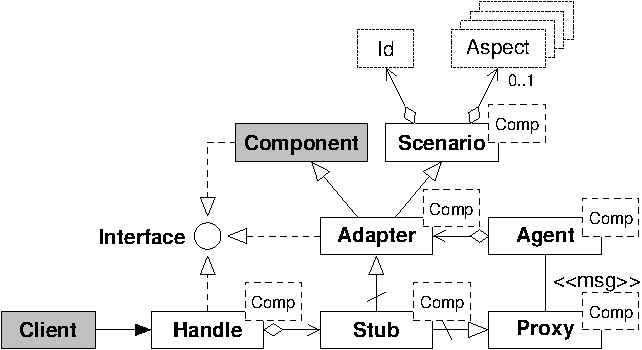
\includegraphics[scale=0.6]{fig/framework}\\
(a) \EPOS{} metaprogrammed framework. \\
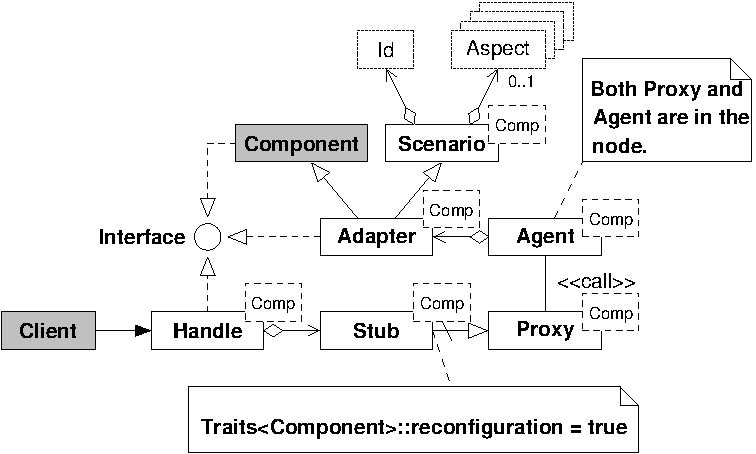
\includegraphics[scale=0.6]{fig/framework-reconf}\\
(b) Framework for software reconfiguration. \\
\end{tabular}
\caption{(a) \EPOS{} metaprogrammed framework overview~\cite{Froehlich:2001}. (b) \EPOS{} metaprogrammed framework for software reconfiguration.}
\label{fig:framework}
\end{figure}

The \stub{} element is a parametrized class responsible for verifying whether the \textit{aspect of remote invocation} is active for that component (the remote invocation aspect is selected by the component through its \textit{Trait Class}~\cite{Stroustrup:1997}). If it is not, the \stub{} will inherit the component's scenario adapter. Otherwise, a stub's specialization, namely \textit{Stub$<$Component, true$>$}, will inherit the component's \proxy{}. Therefore, when \textit{Traits$<$Component$>$::remote = false}, this makes \handle{} take the scenario adapter as \stub{}, while making it true makes \handle{}  take \proxy{}.

The \proxy{} is responsible for sending a message with the component method invocation to its \agent{}. A message contains the object, method, and class IDs that are used by \agent{} to invoke the correct method, associating them to a method table. The object ID is used to get the correct object before calling the method. The \agent{} receives the message and invokes the method through \adapter{}.

\adapter{} class is responsible for applying the aspects supplied by \scenario{} before and after the real method call. Each instance of \scenario{} consults the component's \textit{Traits} to verify which aspects are enabled for that component, aggregating the corresponding scenario aspect. When an aspect is not selected for the component, an empty implementation is used. In this case, no code is generated in the final system image, as an aspect weaver in traditional Aspect-Oriented Programming (AOP).

The framework structure is totally transparent to applications due to the use of two namespaces: one for applications and another one for the system. At compilation-time, system components are exported to the application's namespace as demonstrated in Figure~\ref{prg:export}. Consequently, a method invocation from application to a system component is done in the same way (\textit{component-$>$method()}), but instead of calling the real method, the call passes through the framework. System components which want to invoke methods from reconfigurable components, must use the application namespace as well (\textit{Application::Component}).

\prg{export}{Exporting a system component to application namespace.}

We have observed in this work that the \proxy{}/\agent{} structure found in the framework creates an indirection level between method invocation from client to system components with the remote aspect enabled, isolating the components and making them memory position independent. In this scenario, from the client perspective, a remote method invocation is carried out without knowing the component location. This isolation could also be applied for a dynamic software reconfiguration, since only the \agent{} framework member is aware of the component memory location. Unlike the remote method invocation aspect, we propose  replacing the method invocation over the network between \proxy{} and \agent{} to a simple method call between them. Consequently, the same indirection level could reside at same address space of a node. Figure~\ref{fig:framework}(b) demonstrates this scenario in the framework structure.

\section{Epos Live Update System (ELUS)}
\label{sec:elus}

In order to perform a safe and correct software reconfiguration without compromising the system, there are three \textbf{main} requirements that must be satisfied~\cite{Polakovic2008}:

\begin{enumerate}
 \item \textbf{Quiescent State: } before executing a software reconfiguration, the system must reach a consistent state, which is named quiescent state. In a multithread environment such as \EPOS{}, a quiescent state of a component is reached when none of the Threads are calling methods from it.

  \item \textbf{State Transfer: } after reaching a quiescent state, the state of the old component (attributes) must be transferred to the new one, when there are attributes. The state transfer can be performed through memory copy from old to new component, by creating a new object and passing attributes' values from the old component to the new object's constructor, or by accessing the \textit{set} and \textit{get} methods from the components.

  \item \textbf{Reference Redirection: } in order to keep the system consistent, references pointing to old component code must be redirected to new component code.
\end{enumerate}

In addition to these requirements, an embedded system has specific restrictions. Therefore, a software reconfiguration mechanism competes for resources with the target embedded system. Thus it should use the minimum amount of resources possible. Consequently, low memory, processing, and power consumptions are \textbf{desirable} requirements 

\subsection{Assumptions}

Based on the software reconfiguration requirements, \ELUS{} defines the following assumptions:

\begin{itemize}
 \item The reconfiguration unit is a component. A component is marked as reconfigurable or not at compile-time, and hence only those marked as reconfigurable can be updated. For those that are not marked as reconfigurable, no overhead (in terms of memory and processing) is added in the final system image. Yet, all system can be marked reconfigurable.

 \item The quiescent state of a component must be reached before executing a reconfiguration. In this way, a reconfiguration will be done consistently and will not disrupt the system behavior.

 \item The system hardware does not change. Both old and new versions of a component execute in the same hardware platform.

 \item It is up to the developer to ensure that the new component code does not remove any method being used by other components during a reconfiguration.

 \item Reconfigurable methods of a component must be declared virtual. When a method is declared virtual, the C++ compiler generates a virtual method table (\textit{vtable}) for objects of that component. This table contains the component methods' addresses. A vtable supports run-time binding, and will be used to redirect the references from old component code to new component code.

 \item The access of a component attribute must exclusively be done by invoking \textit{set} and \textit{get} methods. Thus, the state transfer uses the \textit{get} method to pass attribute values from the old component to the constructor of the new component object. After that, the old component object is deleted.
\end{itemize}

\subsection{Architecture Overview}

An overview of the \ELUS{} architecture is presented in Figure~\ref{fig:architecture_v2.pdf}. The original framework infrastructure was extended to support software reconfiguration. The invocation of a component method of the client (an application or a component) passes through \proxy{} which sends a message to the \agent{}. After the method execution, a message with the return value is sent back to the client. An indirection level is created between the client and the real component, making the \agent{} the only one aware of the component's position in the system memory. The \textsc{OS Box} at \agent{} was added to control the access to the component method through a synchronizer (\textit{Semaphore}) for each component, avoiding the invocation of a component method while it is being reconfigured. It also acts as an entry point for invoking methods of a reconfigurable component, calling an \agent{} method through a methods table. The \agent{} forwards the invocation to the \adapter{} which calls the real component method through the object vtable.

\fig{architecture_v2.pdf}{\ELUS{} architecture overview.}{totalheight=0.2\textheight, width=0.47\textwidth}

The framework is a metaprogram which means that all dependencies between a component and execution scenarios are resolved during the system compilation. Nonetheless, the \proxy{} element is \textit{dissolved} into the client by the compiler. In this way, calls from \proxy{} to \agent{} are done directly from client to OS box. In the generated code, the \proxy{}, \handle{}, and \stub{} elements do not exist.

%\prg{inv}{A component method invocation through the Framework structure after compiling the system.}
\fig{invFlow}{A component method invocation through the Framework structure after compiling the system.}{scale=.6}

Figure~\ref{fig:invFlow} exemplifies a method invocation using the \ELUS{} framework. The application directly calls the OS Box from the main function. The OS Box accesses the \agent{} method through a methods table (\textit{Dispatcher)} and calls the correct method. The \agent{} recovers the received parameters and calls the \adapter{}. Finally, \adapter{} calls the real component method using the object's vtable.

\subsection{ELUS Framework Elements}

The \handle{} \ELUS{} framework element is depicted in Figure~\ref{fig:handle.pdf}. It is responsible for verifying if a component was marked as reconfigurable or not by accessing the component Trait class. It has the same interface (operations) as the component, but method invocations are forwarded to \stub{} (\textit{stub-$>$method()}). The \stub{} element, however, will inherent the \proxy{} element if the reconfiguration is enabled. Otherwise, it will inherent an \adapter{}.

\fig{handle.pdf}{\ELUS{} Handle element.}{scale=.5}

Figure~\ref{fig:proxy_agent.pdf} shows the \proxy{} and \agent{} elements. These elements will only be present if the reconfiguration is enabled for a component. \proxy{} realizes the component methods. It uses the \msg{} class in order to pass a method invocation to \agent{}. When \proxy{} receives a request from \handle{}, it fills out a message by attaching the method and component IDs and parameters in a message.

%\figspan{proxy_agent.pdf}{\ELUS{} Proxy and Agent elements.}{scale=.5}
\fig{proxy_agent.pdf}{\ELUS{} Proxy and Agent elements.}{totalheight=0.28\textheight, width=0.48\textwidth}

The \msg{} class offers an interface for attaching and detaching parameters and return values (methods \textit{in} and \textit{out}). These methods are also used in \agent{} to recover parameters or to return a value. The invoke \msg{} method calls the \textsc{OS Box} function, which uses an array (\textit{Dispatcher}) in order to deliver the call to \agent{}. Figure~\ref{prg:dispatcher} shows the dispatcher and OS Box implementations.

\prg{dispatcher}{OS Box and Dispatcher implementations.}

The \agent{} element is responsible for calling the \adapter{} methods and reconfiguring a component through the \textbf{update} method. A Thread, called \textsc{Reconfigurator}, created during the system bootstrapping, receives a reconfiguration request and the new component code from the network (RS-232 or radio for example). This request is sent to the \agent{} in the form of a \msg{} using the \etp{} (\ETP{}) through the \textsc{OS Box} as well.

\subsection{Elus Transport Protocol (ETP)}

\etp{} (\ETP{}) is a protocol for receiving reconfiguration messages. Figure~\ref{fig:etp} shows these messages. A control field identifies the reconfiguration type. There are six possible reconfigurations: (a) those for adding a method into a component; (b) those for removing a method from a component; (c) those for updating a component; (d) those for updating a specific memory address; (e) those for updating the application; and (f) those for adding an attribute into a component.

\begin{figure}
\centering
\begin{tabular}{cc}
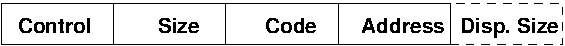
\includegraphics[scale=0.5]{fig/msg_add_en} & \\
(a) & \\
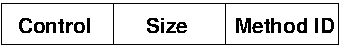
\includegraphics[scale=0.5]{fig/msg_rem_en} &
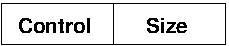
\includegraphics[scale=0.5]{fig/msg_atr_en} \\
(b) & (f)\\
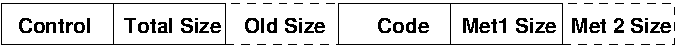
\includegraphics[scale=0.5]{fig/msg_upd_en} & \\
(c) & \\
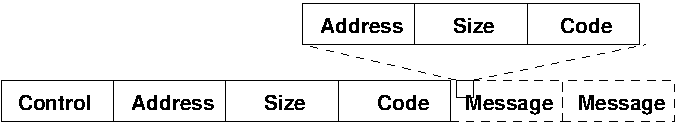
\includegraphics[scale=0.5]{fig/msg_end_en} & \\
(d) & \\
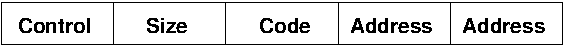
\includegraphics[scale=0.5]{fig/msg_app_en} & \\
(e) & \\
\end{tabular}
\caption{ETP messages overview. (a) Method adding message (b) Method remove message (c) Component update message (d) Address update message (e) Application update message (f) Attribute adding message.}
\label{fig:etp}
\end{figure}

\agent{} uses the control field in order to identify which reconfiguration type is sent by the \textsc{Reconfigurator}. The control field also identifies if the new component or method code is larger than the old one. If it is, \agent{} allocates new memory for the new code. If it is not, the \agent{} overwrites the old code. \ETP{} is a simple protocol, allowing an easy integration with data dissemination protocols~\cite{stathopoulos03remote, deluge, mnp}, for instance.

\subsection{Reconfiguration Process}

The reconfiguration process is done by the \agent{} \textbf{update} method, which receives a \msg{} in the \ETP{} format. Figure~\ref{fig:updateAgent.pdf} exemplifies a component update reconfiguration. The \textsc{Reconfiguration} sends an \ETP{} message to \textsc{OS Box} informing of a component update. The \textsc{OS Box} reaches the quiescent state by calling a semaphore \textit{p()} operation. After that, the \agent{} reads the message fields (method \textit{in}), and recovers the object(s) associated with the component ID and its vtable address (\textit{*addr = *reinterpret\_cast$<$unsigned int$>$($\&$t)}). The control field stores information if the new component code is larger than the old one. If so, the \agent{} allocates a memory space for the new code through a \textsc{Code Manager}. Otherwise, the new code is written in the same position of the old one. In the end, \agent{} updates the methods addresses in the vtable and releases the component semaphore by calling the \textit{v()} operation.

\fig{updateAgent.pdf}{Sequence diagram of the Agent update method when performing a component updating.}{totalheight=0.35\textheight, width=0.48\textwidth}

\textsc{Code Manager} is a class that manages the system code memory. It exports a simple interface to components which want to allocate, release, write, or read bytes to or from the code memory. \textsc{Code Manager} is important because it abstracts memory dependencies among platforms (e.g. harward or von neuman architecture), meaning that each architecture should have its own \textsc{Code Manager}.

In order to support an application update, we implemented a special component, called \textsc{Application Update}. This component is responsible for receiving an application update request in \ETP{} format and updating the application code as needed. It can be reconfigurable as well. \textsc{Application Update} uses two \ETP{} messages: application update message and address update message. The control field identifies which updating type is being requested.

%\fig{updateApp.pdf}{Update\_Application component sequence diagram.}{totalheight=0.4\textheight, width=0.42\textwidth}

%Figure shows the Update\_Application component sequence diagram when performing an updating. Initially, it verifies what is the message type and reads the message parameters as the message type. The application update message (code 0x8) informs the component that the new application code is larger than old. Thus, the component allocates new memory space and writes the new code to that space. The message also carries all addresses that were referencing the old code, and update these addresses with the new allocated memory address. If the received message is an address update message (code 0x7), which means that the new application code is less or equal than old, the received code is written in the same application position.

A new component code is compiled, linked with the generated system image, and its code sent over the network. The new component code is linked using the \textsc{OS Box} address, which is the entry point for calling methods through the framework infrastructure. Therefore, the \textsc{OS Box} is the only system element that \textbf{is not} reconfigurable.
 %Thus, there is an unique function that is not reconfigurable. This function is the \textsc{OS Box}, which is the entry point for calling methods through the framework infrastructure. In fact, this function always does the same instructions. It receives a message with the component and methods IDs, access the Dispatcher for recovering the \agent{} method, and call this method.


\section{Experimental Evaluation}
\label{sec:evaluation}

\subsection{Synthetic Benchmark Configuration}

In order to corroborate design choices, we have evaluated \ELUS{} in terms of three metrics: memory consumption, overhead associated with indirection level composed by the framework structure and virtual method table, and time spent in a reconfiguration. We have used GNU g++ compiler 4.0.2 and GNU objdump tool 2.16.1 to generate the system and analyze these metrics, respectively.

The platform used was the Mica2 mote~\cite{mica2}, composed by an 8-bits AVR Atmega128 microcontroller, with 4KB of RAM memory, 128KB of flash memory, 4KB of EEPROM, and a set of peripherals including radio communication. 
%This is the same platform used in the related work.

\subsection{Memory Footprint}
\label{sec:memory}

In the first evaluation, the reconfiguration support was enabled only in the \textit{Chronometer} component that has 8 reconfigurable methods~\cite{timer}. The objective was to measure the memory overhead added by the \ELUS{} infrastructure. Table I presents the memory consumption of the \ELUS{} elements in this scenario. The framework has needed about 2.6kb of code memory, 43 bytes of data for \textit{Dispatcher} and control attributes, and 52 bytes of non-initialized data for hash table in the \scenario{} framework element. \textsc{Reconfiguration} needs 70 bytes of data due to a buffer for receiving data from the network. This buffer was configured with size of 40 bytes. The \textsc{Application Update} component uses 210 bytes of code memory. The total memory consumption for this case is about of 3.5Kb of code memory and 148 bytes of data.

\begin{table}[ht]
\centering
\footnotesize{
\caption{\ELUS{} memory consumption.} 
\begin{tabular}{|c|c|c|c|c|}\hline
\textbf{\ELUS{}} & \multicolumn{4}{c|}{\textbf{Section Size (bytes)}} \cr
\cline{2-5}
\textbf{Elements} & \textbf{.text} & \textbf{.data} & \textbf{.bss} & \textbf{.bootloader} \cr
\hline
\textbf{Reconfigurator} 	& 410 & 0 & 70 & 0  \cr\hline
\textbf{Code Manager} 		& 16 & 0 & 2 & 375  \cr\hline
\textbf{App. Update} 		& 210 & 0 & 0 & 0  \cr\hline
\textbf{OS Box} 		& 76 & 0 & 0 & 0  \cr\hline
\textbf{Framework} 		& 2620 & 43 & 52 & 0  \cr\hline
\hline
\textbf{Total} & 3452 & 43 & 124 & 375 \cr
\hline
\end{tabular}
}
\label{tab:memory}
\end{table}

The second memory benchmark evaluated the memory consumption of individual methods in the framework for a generic component. This test only considers the memory consumption of the framework, disregarding the memory needed by the component itself. The objective was to measure the memory overhead added for a component when it is marked as reconfigurable. Table II shows the evaluation.

\begin{table}[ht]
\centering
\footnotesize{
\caption{Memory consumption of individual methods in \ELUS{} framework.}
\begin{tabular}{|c|c|c|}\hline
\textbf{Framework} & \multicolumn{2}{c|}{\textbf{Section Size (bytes)}} \cr
\cline{2-3}
\textbf{Method} & \textbf{.text} & \textbf{.data} \cr
\hline
Create				& 180  & 0  \cr\hline
Destory 			& 138  & 0  \cr\hline
Method without parameter  	& 94 & 0  \cr
and return value 		& & 	\cr\hline
Method with one parameter   	& 98 & 0  \cr
and without return value 	& &  \cr\hline
Method without parameter 	& 112  & 0  \cr
and with return value 		& &  \cr\hline
Method with one parameter  	& 126 & 0  \cr
and return value 		& &  \cr\hline
Update	 			& 1250  & 0   \cr\hline
Dispatcher 			& 0  & 2 X (methods)  \cr\hline
Semaphore 			& 0  & 18   \cr\hline
\hline
\textbf{Minimal Size}  & 1662 & 26 \cr
\hline
\end{tabular}
}
\label{tab:per}
\end{table}

There are three methods that are always added by the framework: \textit{create} (constructor), \textit{destroy} (destructor) and \textit{update} (responsible for reconfiguring the component). Moreover, there is a table of \agent{} methods (\textit{Dispatcher}). Each method inside \textit{Dispatcher} occupies 2 bytes. The other values present the overhead associated with a specific method of a component. For instance, if a component method passes one argument and receives a return value, there is memory consumption implicitly due to the \msg{} structure for passing the arguments and return value. Also, each component must have a semaphore to control its access, which occupies 18 bytes in the data section. Thus, the minimal memory consumption (with create, destroy, update, and one method without parameters and return value) for a reconfigurable component is about 1.6Kb of code and 26 bytes of data. Equation 1 can be used for calculating the total framework memory consumption for a component.

\label{for:size}
\begin{align}
Size_{c} = \sum_{i=1}^n (Method_{i}) + Create + Destroy + Update
\end{align}

\subsection{Method Invocation Overhead}
\label{sec:overhead}

The indirection level from the application to a component method creates an overhead. Before calling the real method, \agent{} should get the arguments from \msg{}, recover the object from the hash table, and finally call the method using the object's vtable. Figure~\ref{fig:invTime.pdf} presents a comparison among four types of methods: (i) without receiving parameters and returning value; (ii) without receiving parameters, but returning value; (iii) receiving one parameter, but without returning value; and (iv) receiving one parameter and returning value. For each type, there is a comparison among \ELUS{}, using an object vtable, and through a regular method invocation. The method invocation overhead was about 10 times worse than using a virtual method table. As will be shown in Section~\ref{sec:analysis}, this overhead is lower than in related work.

\fig{invTime.pdf}{Comparison of invocation time among a regular method invocation, through vtable and through \ELUS{}.}{totalheight=0.2\textheight, width=0.45\textwidth}

\subsection{Reconfiguration Time}
\label{sec:reconfTime}

Table III presents the reconfiguration time in two component update scenarios, when the new component code is larger than old and when the new component code is less or equal to the old one. In this test the time spent in the \textsc{Reconfigurator} for calling the \textsc{OS Box}, the time spent in the \textsc{OS Box} for accessing the \textit{Dispatcher} and calling the \agent{} update method, and the time spent by the \agent{} update method on getting the arguments from message and executing a reconfiguration were considered. The time needed for receiving data from the network in the \textsc{Reconfigurator} and the time for writing data to the flash memory were not considered because these times are also not used in the related work.

\begin{table}[ht]
\centering
\footnotesize{
\caption{Time (in processor cycles) for a component reconfiguration.}
\begin{tabular}{c|c|c|}
\cline{2-3}
 & \multicolumn{2}{|c|}{\textbf{Time (in cycles)}}\cr
\cline{2-3}
 & \textbf{Update} & \textbf{Update} \cr
& \textbf{same position} & \textbf{new position} \cr
\cline{1-3}
\multicolumn{1}{|c|}{\textbf{Agent Update}} & 238 & 290 \cr
\hline
\multicolumn{1}{|c|}{\textbf{Reconfigurator}}  & 65 & 65 \cr
\hline
\multicolumn{1}{|c|}{\textbf{OS Box}} & 59 & 59 \cr
\hline
\hline
\multicolumn{1}{|c|}{\textbf{Total}}	& 362 & 414 \cr\hline
\end{tabular}
}
\label{tab:time}
\end{table}

\textsc{Reconfigurator} consumes 65 processor cycles to call the \textsc{OS Box}. The \textsc{OS Box} needs 59 cycles for calling the \textit{p()} and \textit{v()} semaphore operations, and \agent{} update method. Finally, the update method spends 238 cycles performing an update in the same position as the old component code, and 290 cycles to update a component with new code larger than the old one.

\section{Result Analysis}
\label{sec:analysis}

This section discusses the \ELUS{} results by comparing them to related work. Primarily, it will be presented the main operating systems that support software reconfiguration in embedded systems domain and after they will be compared to \ELUS{}.

\subsection{Related Work}
\label{sec:related}

\textsc{TinyOS} is considered the most popular OS for WSNs. It is an event-driven OS and originally does not support software reconfiguration~\cite{hill00system}. However, several works have been done in order to support reconfiguration in \textsc{TinyOS}~\cite{deluge, flexcup, mate}. \textsc{MantisOS} is another well-known OS for WSNs, but does not support software reconfiguration~\cite{mantis}.

\textsc{Nano-Kernel} allows dynamic reconfiguration of application
and kernel components by decoupling the kernel data objects from
the logical kernel algorithms~\cite{Bagchi2008}. The kernel address space is split up
in two parts, the nano-kernel core and kernel devices, such as scheduler
and memory manager. The nano-kernel core is responsible for creating
an indirection level between application and kernel devices.
In this way, when an application invokes a function from a kernel device
or a kernel device invokes a function from another kernel device, the
nano-kernel core redirects the call to the appropriate kernel device
and returns the result to the caller. The nano-kernel core and the
kernel devices communicate through a specific interface. In system boot, all kernel devices 
need to be loaded, and their interfaces need to be initialized with the appropriate methods. As the nano-kernel
core receives all method calls from the interface, it must check
if the kernel device has permission to access the data object, thus
incurring an overhead to the system.

\textsc{RETOS} implements a mechanism for dynamic reconfiguration of system
modules through a dynamic memory relocation and linking at run-time~\cite{Cha2007}.
The relocation process extracts the information from global variables
and functions at compile-time, creating meta-information (hardware-dependent
information) about the module that is being updated. This information
is placed in a \textsc{RETOS} file format that is used by the system kernel 
to replace every accessible address of a module when performing
a module load. The OS also keeps a table that allows modules and
applications to access other module functions. A module registers,
unregisters, and accesses functions through this table. On the other
hand, an application accesses the module function through a system
call which invokes the required function by accessing this table.

\textsc{Contiki} is an OS for WSNs
that implements special processes, called \emph{services}, which
provide functionality to other processes~\cite{dunkels04contiki}.
Services can be replaced at run-time through a \emph{stub interface}
that is responsible for redirecting function calls to a \emph{service
interface}, which holds the actual pointers to the functions
implementing the corresponding services.  The \emph{service interface}
also keeps track of versions during updates. Contiki is not full reconfigurable,
that is, it only allows the updating of some system parts.

\textsc{SOS} is an operating system for sensor networks that allows
nodes to be updated on-the-fly~\cite{sos}. The OS is
built around modules that can be inserted, removed, or replaced at
run-time. By using relative calls, the code in each module becomes
position independent.  References to functions and data outside the
scope of a module are implemented through an indirection table and, in
some cases, are simply not allowed. \ELUS{} is conceptually
similar to the previously presented works, but the framework
infrastructure takes advantage of static
metaprogramming techniques to eliminate part of the overhead
associated with indirection tables, thus yielding a slimmer and configurable mechanism,
and also achieving application transparency. Table~\ref{tab:reconf2}
shows an overview of the reconfiguration process in the analyzed embedded
operating systems.

\begin{table}[ht]
\centering
\caption{Reconfiguration process characteristic in the analyzed embedded OSs.}
\footnotesize{
\begin{tabular}{{|c|p{5.8cm}|}}
\hline
\textbf{OS} & \multicolumn{1}{c|}{\textbf{Reconfiguration Process}} \cr\hline
\textsc{TinyOS}      &  \multicolumn{1}{c|}{No direct support} \cr\hline
\textsc{MantisOS}    & \multicolumn{1}{c|}{There is no support} \cr\hline
\textsc{Nano-Kernel} & \multicolumn{1}{c|}{Reconfigurable modules} \cr\hline
\textsc{RETOS}       & \multicolumn{1}{c|}{Dynamic relocation and runtime linking} \cr\hline
\textsc{Contiki}     & \multicolumn{1}{c|}{Reconfigurable modules} \cr\hline
\textsc{SOS}         & \multicolumn{1}{c|}{Reconfigurable modules} \cr\hline
%Think       & \multicolumn{1}{c|}{Modelo reflexivo (Fractal)} \cr\hline
\textsc{\textbf{EPOS/ELUS}} & \multicolumn{1}{c|}{\textbf{Selected reconfigurable components}} \cr\hline
\end{tabular}
}
\label{tab:reconf2}
\end{table}

\subsection{Discussion}
\label{sec:disussion}

The minimum \ELUS{} memory consumption is about 1.6Kb of code and 26 bytes of data per system component. \textsc{Contiki} needs 6Kb of code and 230 bytes of data~\cite{dunkels04contiki}. \textsc{SOS} occupies more than 4Kb of code for managing the modules and the module table occupies 230 bytes of data. \ELUS{} presents good performance due to static metaprogramming, which solves all dependencies between the framework, components, and application at compile-time. Moreover, \ELUS{} allows the developer to choose the reconfigurable components without imposing overhead in the final system instance. Therefore, the generated system only contains the code and data really necessary.

Regarding the method invocation overhead, \textsc{SOS} takes 21 cycles for calling a function of a reconfigurable module and takes 12 cycles for calling a kernel function. However, the communication between modules (data exchange) is carried out by sending and receiving messages in a buffer, which takes 833 cycles~\cite{sos}. \textsc{Contiki} has a worse performance because the stub should find the service interface before calling a function of a reconfigurable module. This is done by comparing a string of characters. After that, the function is accessed by a function pointer~\cite{dunkels04contiki}. In a comparison, \textsc{Contiki} was 4 times slower than \textsc{SOS}~\cite{Yi2008}. \textsc{RETOS} and \textsc{Nano-Kernel} also present an overhead associated with the indirection level. \ELUS{} has the advantage of using the \message{} framework structure for passing arguments and return value, which is 7 times faster than \textsc{SOS}.

Finally, in a reconfiguration, \textsc{SOS} removes the old module and registers the new module and its event handler. It takes 621 cycles to perform these activities, disregarding the times for receiving the data from network and writing the code to flash memory~\cite{Yi2008}. \textsc{Contiki} also has a similar performance. It starts sending a message for removing the service interface, makes the state transfers between the old and new modules, and ends registering the new service interface. \textsc{RETOS} uses dynamic relocation and linking at run-time. There are meta-data that contain information about modules. These meta-data are transmitted together with the new code, which increase the data transmitted over the network and the reconfiguration time. \ELUS{} does not need to register and unregister components at run-time. All dependencies are solved at compile-time. It takes about 500 cycles for performing a reconfiguration. \ELUS{} also decreases the data sent to network by using the \etp{}, which needs from 2 to 6 extra bytes.



\section{Conclusions}
\label{sec:conc}
This paper presented \ELUS{}, a low-overhead OS infrastructure for resource-constrained embedded systems. \ELUS{} was developed
around \EPOS{} component framework, which was modified in order to
enable confinement and isolation of system components in physical
modules, thus making them memory position independent. The infrastructure also
allows the developer to choose at compile-time which components can be reconfigurable. For those components marked as not reconfigurable, no overhead is added in the final system image. Moreover, \ELUS{} is totally transparent for applications and by using the \etp{}, the software reconfiguration becomes simple and easy to integrate with other protocols, such as a data dissemination protocol.

Results have shown that \ELUS{} consumes less memory, adds a lower overhead, and has a better reconfiguration time in comparison to related work. The next step in the project is to integrate a data dissemination protocol with \ELUS{} in order to support code distribution over the network.

\bibliographystyle{IEEEtran}
\bibliography{references}

\end{document}


